\documentclass{article}
\renewcommand\familydefault{\sfdefault} 
\usepackage{graphicx} % Required for inserting images
\usepackage{enumitem}
\usepackage{tikz}
\usetikzlibrary{shapes.geometric, arrows}

\tikzstyle{startstop} = [rectangle, rounded corners, 
minimum width=3cm, 
minimum height=1cm,
text centered, 
draw=black, 
fill=red!30]

\tikzstyle{process} = [rectangle, 
minimum width=3cm, 
minimum height=1cm, 
text centered, 
text width=3cm, 
draw=black, 
fill=orange!30]

\tikzstyle{decision} = [diamond, 
minimum width=3cm, 
minimum height=3cm, 
text width=1.5cm,
text centered, 
draw=black, 
fill=green!30]
\tikzstyle{arrow} = [thick,->,>=stealth]

\newlist{questions}{enumerate}{2}
\setlist[questions,1]{label=RQ\arabic*.,ref=RQ\arabic*}
\setlist[questions,2]{label=(\alph*),ref=\thequestionsi(\alph*)}


\title{Project plan for Mutation-Based Accuracy Improvements in Neural Networks using Spectrum-Based Fault Localization\\
\textit{Mutationsbasierte Genauigkeitsverbesserungen in neuronalen Netzwerken unter Nutzung spektrumbasierter Fehlerlokalisierung.}}
\author{Lennart Mühlhahn}
\date{\today}
\usepackage[style=ieee]{biblatex}
\addbibresource{export.bib}

\usepackage{hyperref}
\begin{document}

\maketitle

\section{Adapt DeepFault Functions}
Adapting the needed DeepFault functions (excluding suspiciousness-guided input synthesis) from the DeepFault GitHub repo \cite{eniser_deepfault_2019} \cite{eniser_deepfault_2023} to the new TensorFlow version. Furthermore, add a function to choose nodes at random.
\section{Implement mutation functions}
Functions for the following mutations:
\begin{itemize}
    \item weight and bias mutations
    \begin{itemize}
        \item random
        \item by a fixed value
        \item with a fixed value
    \end{itemize}
    \item remove nodes
    \begin{itemize}
        \item remove by slicing
        \item set bias to zero
        \item add a “sieve” layer
    \end{itemize}
\end{itemize}
These functions need to be modified according to the findings of the DeepFault suspicious neuron identification.
\section{Setup experiments}
Implement a CNN and DNN based on the Fashion-MNIST dataset \cite{xiao_fashion-mnist_2017} for experimenting. Create a container for conducting experiments.
\section{Perform experiments}
The experiments will try to modify suspicious nodes or delete suspicious nodes. I will try this until I get no more accuracy gains on the test data or a predefined number of modified nodes is reached. For the training one epoch will be performed and evaluated, but not used for further mutations, just for the evaluation.\\
\begin{center}
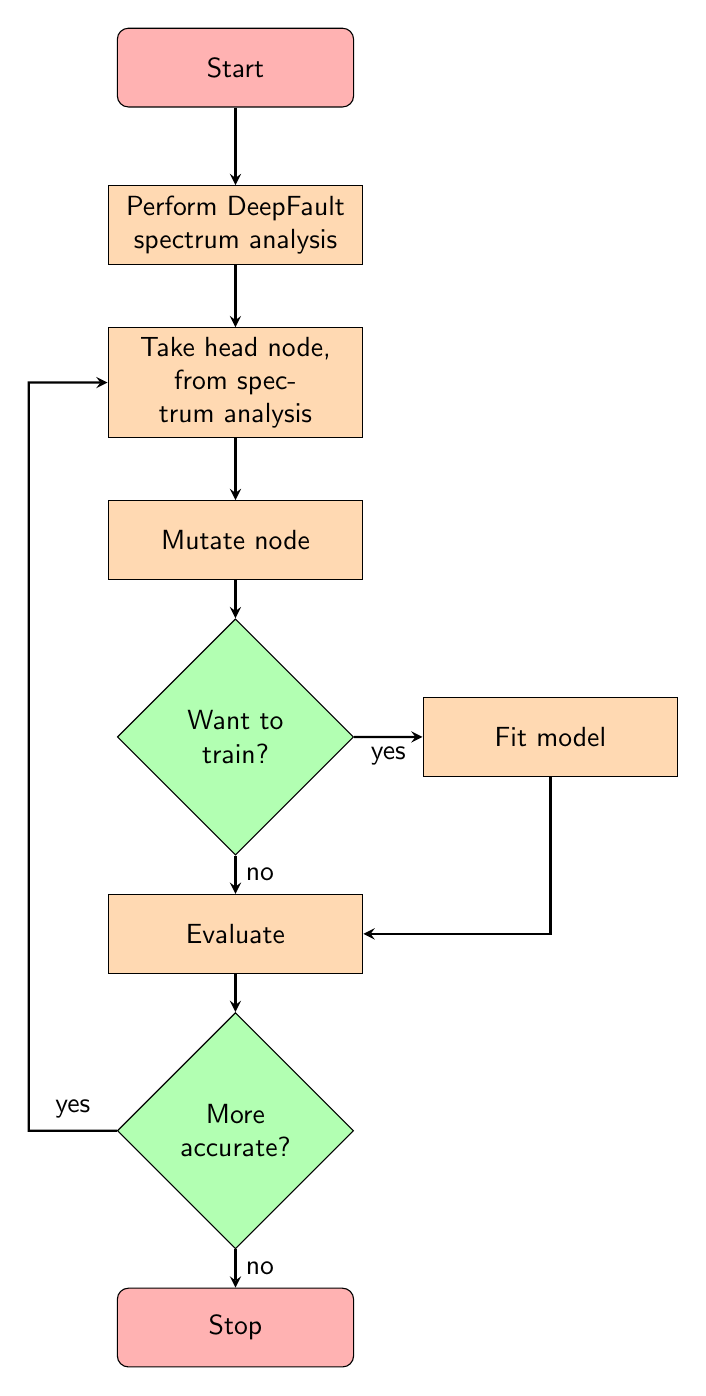
\begin{tikzpicture}[node distance=2cm, scale=0.75]

\node (start) [startstop] {Start};
\node (pro1) [process, below of=start] {Perform
DeepFault
spectrum analysis};
\node (pro2) [process, below of=pro1] {Take head node, from spectrum analysis};
\node (pro3) [process, below of=pro2] {Mutate node};
\node (dec1) [decision, below of=pro3, yshift=-0.5cm] {Want to train?};
\node (pro4a) [process, below of=dec1, yshift=-0.5cm] {Evaluate};
\node (pro4b) [process, right of=dec1, xshift=2cm] {Fit model};
\node (dec2) [decision, below of=pro4a, yshift=-0.5cm] {More accurate?};
\node (stop) [startstop, below of=dec2, yshift=-0.5cm] {Stop};

\draw [arrow] (start) -- (pro1);
\draw [arrow] (pro1) -- (pro2);
\draw [arrow] (pro2) -- (pro3);
\draw [arrow] (pro3) -- (dec1);
\draw [arrow] (dec1) -- node[anchor=north] {yes} (pro4b);
\draw [arrow] (pro4b) |- (pro4a);
\draw [arrow] (dec1) -- node[anchor=west] {no} (pro4a);
\draw [arrow] (pro4a) -- (dec2);
\draw [arrow] (dec2) -- node[anchor=west] {no} (stop);
\draw [arrow] (dec2) -- node[anchor=south, above=1pt] {yes} ++(-3.5,0) |- (pro2);
\end{tikzpicture}
\end{center}
\section{Draft introduction}
\section{Draft main chapter}
\section{Draft background chapter}
\begin{itemize}
    \item Deep neural networks
    \item DNN testing and verification 
    \item Mutation-based testing
    \item Spectrum analysis
\end{itemize}
\section{Draft experimental results chapter}
\section{Draft conclusion}
\section{Revise chapters}
\section{Write abstract}
\section{Print Thesis}

\section*{Research Questions}
\begin{questions}
    \item Could the mutation of faulty neurons improve the quality and reliability  of a Deep Neural Network?
    \item Could the mutation of faulty neurons during training improve the quality and reliability of a Deep Neural Network?
    \item Which mutations are the most promising for improvement?
    \item Which combinations of mutations are the most promising?
    \item Which suspiciousness measure is the most promising for improving a Deep Neural Network?
    \item Are the suspiciousness measures more accurate than random choosing?
\end{questions}
\section*{Proposed Title}
\printbibliography

\end{document}
